\chapter{Modelli di anomaly detection}

\section{Approccio ibrido e multilivello al rilevamento di anomalie}
Nel monitoraggio intraoperatorio continuo, l'identificazione precoce di deviazioni fisiologiche critiche costituisce un obiettivo primario per la sicurezza del paziente. La dinamica biologica di un organismo sottoposto ad anestesia generale e a stimoli chirurgici è tuttavia estremamente complessa ed eterogenea: gli eventi avversi possono manifestarsi sia sotto forma di repentine cadute pressorie sia come graduali e insidiose dissociazioni tra parametri vitali multipli.

Per intercettare questo ampio spettro di condizioni, il presente progetto non si affida a un'unica tecnica di analisi, bensì implementa un approccio ibrido multilivello fondato su quattro metodologie complementari:
due regole cliniche deterministiche dominio-specifiche, formulate sulla base delle evidenze della letteratura medica (lo \textbf{Shock Index} e la condizione di ipotensione severa);
due algoritmi di \textbf{machine learning} non supervisionato capaci di operare sullo spazio congiunto delle serie storiche, segnatamente l'algoritmo ad alberi \textbf{Isolation Forest} e un modello neurale ricorrente basato su \textbf{LSTM Autoencoder}.

La complementarità di questo schema risponde a una precisa motivazione clinica e ingegneristica: le regole cliniche hanno una solida giustificazione fisiopatologica e forniscono riscontri trasparenti e immediatamente comprensibili dal personale medico, ma falliscono nell'identificare anomalie multivariate sfumate che precedono l'evento conclamato; al contrario, i modelli di \textbf{machine learning} non supervisionato eccellono nel riconoscere correlazioni inattese e configurazioni atipiche ad alta dimensionalità, sebbene necessitino di una contestualizzazione per distinguere gli artefatti statistici dalle vere emergenze cliniche.

\section{Regole cliniche dominio-specifiche}
Le regole cliniche implementate nello script \texttt{src/detection/detector.py} operano direttamente sulle grandezze fisiologiche archiviate nel livello \textbf{Gold}, valutando soglie note nella pratica anestesiologica.

\subsection{Shock Index clinico}
Lo \textbf{Shock Index} ($SI$) è un indicatore emodinamico adimensionale ampiamente utilizzato nei reparti di rianimazione e pronto soccorso per la valutazione tempestiva del rischio di shock ipovolemico, emorragico o cardiogeno. Esso è definito matematicamente come il rapporto tra la frequenza cardiaca ($HR$) e la pressione arteriosa sistolica ($SBP$):
$$SI = \frac{\text{Solar8000\_HR}}{\text{Solar8000\_NIBP\_SBP}}$$

In un soggetto adulto sano in condizioni stazionarie di riposo, il valore normale dello \textbf{Shock Index} oscilla tra $0.5$ e $0.7$. Quando la gittata sistolica cala a seguito di un'emorragia o di una vasodilatazione indotta dai farmaci anestetici, il sistema nervoso autonomo tenta di compensare aumentando la frequenza cardiaca (tachicardia riflessa) mentre la pressione sistolica tende a diminuire. Il modulo contrassegna come anomalo qualsiasi istante temporale in cui si verifichi la condizione:
$$SI > 0.9$$
Il superamento di questa soglia testimonia il fallimento dei meccanismi fisiologici di compenso e segnala un'instabilità emodinamica imminente che richiede un'immediata infusione di fluidi o l'infusione di vasopressori.

\subsection{Ipotensione severa}
La seconda euristica clinica mira a identificare stati di grave compromissione perfusiva e ipossia cellulare. La regola valuta la compresenza simultanea di una pressione arteriosa media insufficiente e di una desaturazione d'ossigeno periferico:
$$\text{Solar8000\_NIBP\_MBP} < 65 \text{ mmHg} \quad \land \quad \text{Solar8000\_PLETH\_SPO2} < 90\%$$

Il mantenimento di una pressione arteriosa media ($MBP$) al di sopra di $65$ mmHg è universalmente riconosciuto nelle linee guida cliniche come la soglia minima necessaria per garantire l'autoregolazione del flusso ematico nei distretti cerebrale e renale. Quando tale ipoperfusione si associa a una caduta della saturazione al di sotto del $90\%$, l'organismo entra in una condizione di grave sofferenza ipossico-ischemica. La coincidenza temporale dei due segnali costituisce un allarme di massima priorità in sala operatoria.

\section{Ingegnerizzazione delle feature temporali}
Per consentire agli algoritmi di \textbf{machine learning} di catturare non soltanto i valori istantanei dei parametri ma anche la dinamica evolutiva e la tendenza temporale delle serie biometriche, la procedura esegue una fase di estrazione di feature temporali derivate.

A partire dal segnale della frequenza cardiaca (\texttt{Solar8000/HR}), che presenta la cadenza di campionamento più continua e regolare a frequenza di 1 Hz, vengono calcolate tre feature dinamiche fondamentali. Indicando con $x_t$ il valore della frequenza cardiaca all'istante temporale $t$ (in secondi) e con $W = 5$ campioni l'ampiezza della finestra temporale retrospettiva, le metriche vengono definite formalmente come:
la media mobile a cinque campioni (\texttt{HR\_rolling\_mean}), che attenua le micro-oscillazioni e gli artefatti ad alta frequenza senza introdurre ritardi significativi:
$$\mu_t = \frac{1}{W} \sum_{k=0}^{W-1} x_{t-k}$$
la deviazione standard mobile a cinque campioni (\texttt{HR\_rolling\_std}), che quantifica la dispersione e l'instabilità istantanea del battito cardiaco nel brevissimo termine:
$$\sigma_t = \sqrt{\frac{1}{W-1} \sum_{k=0}^{W-1} (x_{t-k} - \mu_t)^2}$$
la differenza prima (\texttt{HR\_delta}), che misura la velocità istantanea di accelerazione o decelerazione del ritmo cardiaco:
$$\Delta x_t = x_t - x_{t-1}$$

L'introduzione di $\Delta x_t$ riveste un ruolo fisiologico cruciale: una repentina variazione positiva di $\Delta x_t$ (oltre 10--15 bpm in un singolo secondo) riflette una scarica adrenergica massiva indotta da un risveglio intraoperatorio o da uno stimolo algico chirurgico acuto, mentre un crollo improvviso testimonia un riflesso vagale o un blocco atrioventricolare.

Al fine di garantire l'assoluta correttezza metodologica, il calcolo di queste finestre mobili viene vincolato al raggruppamento per singolo paziente mediante la trasformazione \texttt{df.groupby("case\_id")}. Questo accorgimento impedisce rigorosamente che i confini temporali di un caso clinico si sovrappongano a quelli del caso successivo, scongiurando qualsiasi contaminazione analitica tra pazienti differenti nei punti di transizione.

Il vettore complessivo delle feature impiegato dai modelli di \textbf{machine learning} comprende otto grandezze numeriche: le cinque metriche vitali originarie (frequenza cardiaca, saturazione d'ossigeno e le tre componenti pressorie) affiancate dalle tre feature dinamiche derivate sulla frequenza. Al contrario, la variabile \texttt{nibp\_age\_s} calcolata nel livello \textbf{Silver} viene deliberatamente esclusa dal vettore; essa rappresenta infatti un metadato di governance attestante la freschezza temporale della misura e non una proprietà biologica intrinseca del paziente.

\section{Modelli di machine learning non supervisionato}
L'approccio basato sull'apprendimento non supervisionato prescinde dalla presenza di etichette a priori e mira a identificare pattern anomali nello spazio delle otto feature biometriche.

\subsection{Isolation Forest}
Il primo algoritmo impiegato è l'\textbf{Isolation Forest}, un metodo di ensemble basato su alberi decisionali isolanti (\textbf{iTree}) particolarmente efficace per serie storiche ad alta dimensionalità.

Il principio teorico dell'algoritmo sfrutta le proprietà geometriche delle anomalie: i punti anomali sono pochi rispetto alla popolazione complessiva e tendono a posizionarsi in regioni periferiche e poco dense dello spazio vettoriale. L'algoritmo partiziona ricorsivamente lo spazio campionario selezionando casualmente una feature ed effettuando un taglio uniforme tra il valore minimo e massimo osservato. Poiché i campioni normali sono densamente raggruppati, essi richiedono un numero elevato di partizioni per essere isolati all'interno di una foglia; al contrario, le istanze anomale, trovandosi isolate nello spazio, vengono separate con pochissimi tagli decisionali.

La lunghezza media del percorso (\textbf{path length}) dalla radice alla foglia attraverso la foresta di alberi fornisce una misura inversa dello score di anomalia. Nello script di produzione, l'algoritmo viene istanziato con una quota di contaminazione teorica fissata al 5\% (\texttt{contamination=0.05}) e con un seme deterministico fissato a 42 per garantire la riproducibilità dei risultati.

\subsection{LSTM Autoencoder neurale (PyTorch)}
Per catturare le interdipendenze sequenziali e la memoria a lungo termine dei segnali fisiologici, è stato progettato e implementato un modello di deep learning basato su reti ricorrenti: l'\textbf{LSTM Autoencoder}, realizzato mediante la libreria PyTorch.

\begin{figure}[ht]
    \centering
    % Diagramma TikZ per l'architettura dell'LSTM Autoencoder con Linear Projection Layer
\begin{tikzpicture}[
    scale=0.88, transform shape,
    font=\sffamily,
    netNode/.style={
        draw=#1!80!black,
        fill=#1!12,
        rounded corners=6pt,
        line width=1.1pt,
        inner sep=6pt,
        align=center,
        font=\small\bfseries,
        drop shadow={opacity=0.12, shadow xshift=2pt, shadow yshift=-2pt}
    },
    ioNode/.style={
        draw=brandBorder,
        fill=white,
        rounded corners=6pt,
        line width=1.1pt,
        inner sep=6pt,
        align=center,
        drop shadow={opacity=0.10, shadow xshift=2pt, shadow yshift=-2pt}
    },
    pipeArrow/.style={
        -{Stealth[length=3.2mm, width=2.2mm]},
        line width=1.8pt,
        color=brandNavy
    },
    lossArrow/.style={
        -{Stealth[length=3.0mm, width=2.0mm]},
        line width=1.5pt,
        color=brandCyan
    }
]

% ==================== LIVELLO 1: PIPELINE NEURALE (DA SINISTRA A DESTRA) ====================

% 1. Input Window
\node[ioNode, minimum width=2.2cm, minimum height=2.2cm] (input) at (0, 0) {
    \textbf{\color{brandNavy}Input $X$}\\[3pt]
    \footnotesize Finestra 30s\\
    \footnotesize 8 feature\\
    \scriptsize $(B, 30, 8)$
};

% 2. Encoder LSTM
\node[netNode=brandCyan, minimum width=2.3cm, minimum height=2.2cm] (encoder) at (2.8, 0) {
    \textbf{Encoder}\\[2pt]
    \textbf{LSTM}\\[4pt]
    \scriptsize 32 unità\\
    \scriptsize Compressione
};

% 3. Bottleneck Z
\node[netNode=orange, minimum width=2.0cm, minimum height=2.2cm] (bottleneck) at (5.6, 0) {
    \textbf{Bottleneck}\\[2pt]
    \textbf{Latente $Z$}\\[4pt]
    \scriptsize Dimensione: 32\\
    \scriptsize Spazio latente
};

% 4. Decoder LSTM
\node[netNode=brandCyan, minimum width=2.3cm, minimum height=2.2cm] (decoder) at (8.4, 0) {
    \textbf{Decoder}\\[2pt]
    \textbf{LSTM}\\[4pt]
    \scriptsize 32 unità\\
    \scriptsize Decodifica
};

% 5. Linear Projection
\node[netNode=purple, minimum width=2.3cm, minimum height=2.2cm] (linear) at (11.2, 0) {
    \textbf{Linear}\\[2pt]
    \textbf{Projection}\\[4pt]
    \scriptsize \texttt{Linear(32, 8)}\\
    \scriptsize Mappatura $\mathbb{R}^8$
};

% 6. Output Window
\node[ioNode, minimum width=2.2cm, minimum height=2.2cm] (output) at (14.0, 0) {
    \textbf{\color{brandNavy}Output $\hat{X}$}\\[3pt]
    \footnotesize Ricostruzione\\
    \footnotesize 8 canali\\
    \scriptsize $(B, 30, 8)$
};

% Frecce della pipeline neurale
\draw[pipeArrow] (input) -- (encoder);
\draw[pipeArrow] (encoder) -- (bottleneck);
\draw[pipeArrow] (bottleneck) -- (decoder);
\draw[pipeArrow] (decoder) -- (linear);
\draw[pipeArrow] (linear) -- (output);


% ==================== LIVELLO 2: VALUTAZIONE ERRORE E DECISIONE (CENTRATI IN BASSO) ====================

% Blocco Calcolo Errore MSE (Centrato sotto la rete a x=7.0)
\node[
    draw=brandBorder,
    fill=brandSurface,
    rounded corners=7pt,
    line width=1.1pt,
    inner sep=8pt,
    minimum width=7.2cm,
    minimum height=2.0cm,
    align=center,
    drop shadow={opacity=0.10, shadow xshift=2pt, shadow yshift=-2pt}
] (mseBox) at (7.0, -3.2) {
    \textbf{\color{brandNavy}Calcolo errore di ricostruzione (MSE)}\\[3pt]
    \small $\text{MSE}(X, \hat{X}) = (X - \hat{X})^2 \quad \implies \quad \text{Score}_{\text{finestra}} = \max_{\text{canale}}(\text{MSE})$\\[2pt]
    \scriptsize (Valutazione comparativa del peggior segnale fisiologico ricostruito)
};

% Blocco Soglia e Decisione Clinica (Subito sotto MSE a x=7.0)
\node[
    draw=brandEmerald!80!black,
    fill=brandEmerald!10,
    rounded corners=7pt,
    line width=1.1pt,
    inner sep=7pt,
    minimum width=9.2cm,
    minimum height=1.6cm,
    align=center,
    drop shadow={opacity=0.10, shadow xshift=2pt, shadow yshift=-2pt}
] (decisionBox) at (7.0, -5.2) {
    \textbf{\color{brandNavy}Classificazione clinica} \quad
    \footnotesize (Soglia empirica: \textbf{$95^\circ$ percentile} sui sani)\\[3pt]
    \scriptsize $\text{Score}_{\text{finestra}} > \text{Soglia}_{95} \implies$ \textbf{\color{red!80!black}ANOMALIA CLINICA} \qquad\quad
    \scriptsize $\text{Score}_{\text{finestra}} \le \text{Soglia}_{95} \implies$ \textbf{\color{brandEmerald!80!black}STATO NORMALE}
};

% Frecce simmetriche da Input e da Output che convergono in mseBox
\draw[lossArrow] (input.south) -- (0, -2.1) -- (5.2, -2.1) -- ([xshift=-1.8cm]mseBox.north);
\node[fill=white, draw=brandCyan!50, line width=0.7pt, rounded corners=3pt, inner sep=2.5pt, font=\scriptsize\bfseries, text=brandNavy] at (2.6, -2.1) {Segnale reale $X$};

\draw[lossArrow] (output.south) -- (14.0, -2.1) -- (8.8, -2.1) -- ([xshift=1.8cm]mseBox.north);
\node[fill=white, draw=brandCyan!50, line width=0.7pt, rounded corners=3pt, inner sep=2.5pt, font=\scriptsize\bfseries, text=brandNavy] at (11.4, -2.1) {Ricostruzione $\hat{X}$};

% Freccia verticale diretta da MSE verso la Classificazione
\draw[pipeArrow] (mseBox.south) -- (decisionBox.north)
    node[midway, right=4pt, font=\scriptsize\bfseries, text=brandNavy] {Score MSE};

\end{tikzpicture}

    \caption{Architettura vettoriale della rete neurale LSTM Autoencoder con proiettore lineare in TikZ.}
    \label{fig:lstm_arch}
\end{figure}

Come schematizzato nella Figura~\ref{fig:lstm_arch}, l'architettura elabora le serie storiche mediante una struttura simmetrica di tipo \textbf{encoder-decoder}:
il modello riceve in ingresso un tensore tridimensionale di forma $(B, W_s, C)$, dove $B$ rappresenta la dimensione del batch, $W_s = 30$ campioni (corrispondenti a 30 secondi di telemetria continua) è l'ampiezza della finestra scorrevole e $C = 8$ è il numero di canali biometrici standardizzati con punteggio z;
l'encoder è costituito da uno strato ricorrente LSTM a 32 unità nascoste (\texttt{hidden\_size=32}), che riceve la sequenza temporale $X \in \mathbb{R}^{30 \times 8}$ e la comprime progressivamente nel vettore di stato nascosto finale $h_{\text{enc}} \in \mathbb{R}^{32}$. Tale vettore costituisce il \textbf{context vector} compresso, che riassume l'intera dinamica evolutiva del blocco temporale;
per alimentare il decoder, il vettore $h_{\text{enc}}$ viene replicato per 30 passi temporali consecutivi (\textbf{repeat vector}), fornendo a ciascun istante del processo di ricostruzione la medesima rappresentazione globale del contesto;
il decoder è composto da un secondo strato ricorrente LSTM speculare a 32 unità, che elabora la sequenza riprodotta generando gli stati di decodifica $h^{\text{dec}}_t \in \mathbb{R}^{32}$ per ciascuno dei 30 istanti;
un layer di proiezione lineare finale (\texttt{nn.Linear}), posizionato all'uscita del decoder, proietta ciascuno stato nascosto nello spazio continuo originale delle feature: $\hat{X}_t = W_p h^{\text{dec}}_t + b_p$, con pesi $W_p \in \mathbb{R}^{8 \times 32}$ e bias $b_p \in \mathbb{R}^8$. L'introduzione di questo strato lineare si è rivelata determinante: la funzione di attivazione tangente iperbolica nativa delle celle LSTM limita infatti le uscite all'intervallo ristretto $[-1, 1]$, impedendo la corretta ricostruzione di variabili standardizzate con punteggio z che superano tali estremi. Il proiettore lineare elimina questo vincolo consentendo la ricostruzione sull'intero asse reale.

L'architettura della rete in PyTorch, definita mediante la funzione interna \\ \texttt{\_make\_lstm\_autoencoder\_class} nel modulo \texttt{detector.py}, è riportata nel Listato~\ref{lst:lstm_pytorch}.

\begin{lstlisting}[caption={Definizione del modello PyTorch LSTM Autoencoder con proiettore lineare per l'anomaly detection.}, label={lst:lstm_pytorch}]
// Modulo PyTorch implementato in src/detection/detector.py
class LSTMAutoencoder(nn.Module):
    def __init__(self, n_features=8, hidden_size=32, n_layers=1):
        super().__init__()
        # Encoder: comprime la sequenza (B, 30, 8) nello stato nascosto (B, 32)
        self.encoder = nn.LSTM(n_features, hidden_size, n_layers, batch_first=True)
        # Decoder: ricostruisce la sequenza temporale partendo dal vettore latente
        self.decoder = nn.LSTM(hidden_size, hidden_size, n_layers, batch_first=True)
        # Proiettore lineare: mappa lo stato nascosto R^32 nello spazio originale R^8
        self.out = nn.Linear(hidden_size, n_features)

    def forward(self, x):
        # x ha forma (batch_size, sequence_length=30, n_features=8)
        _, (hidden, _) = self.encoder(x)
        # Replicazione del context vector per ciascuno dei 30 timestep
        context = hidden.permute(1, 0, 2).repeat(1, x.size(1), 1)
        output, _ = self.decoder(context)
        return self.out(output)  # dimensione ricostruita: (batch, 30, 8)
\end{lstlisting}

La preparazione dei dati per la rete neurale adotta una rigida politica di segmentazione per paziente mediante la classe \texttt{LSTMAutoencoderDetector}:
i dati vengono raggruppati per \texttt{case\_id} e standardizzati con scala z-score;
la suddivisione delle serie in finestre da 30 secondi viene eseguita mediante la funzione vettoriale senza copia \texttt{np.lib.stride\_tricks.sliding\_window\_view}. Questa operazione genera le viste sulle finestre temporali manipolando unicamente gli offset dei puntatori di memoria (\textbf{strides}), senza allocare o duplicare copie fisiche dell'array in memoria RAM. In questo modo è possibile processare agevolmente oltre 300.000 finestre con un consumo di memoria estremamente contenuto;
il modello viene addestrato con ottimizzatore Adam (tasso di apprendimento $10^{-3}$) e funzione di perdita di errore quadratico medio (MSE) per dieci epoche su un campione rappresentativo uniforme di finestre.

Durante la fase di inferenza, la rete valuta la discrepanza tra la finestra di ingresso $X$ e la corrispondente finestra ricostruita $\hat{X}$. Nel calcolo dell'errore di ricostruzione complessivo della finestra, si è deliberatamente scelto di non utilizzare la media aritmetica dell'errore quadratico medio su tutti gli otto canali. In ambito emodinamico, la mediazione globale introdurrebbe infatti un grave rischio di diluizione: se sette parametri su otto rimangono stabili, una caduta acuta e drammatica di un singolo canale vitale (quale una grave desaturazione $\text{SpO}_2$ al di sotto dell'80\% per ostruzione respiratoria improvvisa) verrebbe attenuata dall'effetto mediato degli altri segnali, non riuscendo a superare la soglia di allarme. Per scongiurare tale evenienza, l'errore della finestra viene definito come il massimo errore quadratico medio osservato tra i canali biometrici:
$$\mathcal{E}(X) = \max_{c \in \{1, \dots, C\}} \left( \frac{1}{W_s} \sum_{t=1}^{W_s} (X_{t,c} - \hat{X}_{t,c})^2 \right)$$
L'errore così ottenuto viene assegnato con precisione all'ultimo istante temporale della finestra scorrevole.

La soglia decisionale di anomalia viene fissata in modo non parametrico al $95^\circ$ percentile della distribuzione empirica degli errori $\mathcal{E}(X)$ su tutte le finestre. I campioni il cui errore di ricostruzione supera tale soglia vengono classificati come anomalie fisiologiche multivariate complesse.

\begin{techbox}[brandCyan]{Principio di sensibilità emodinamica nel deep learning}
L'impiego del massimo errore quadratico medio canale per canale ($\max_c \text{MSE}_c$) garantisce che il modello neurale mantenga una sensibilità elevata anche di fronte a collassi isolati di un singolo parametro vitale (es. ipossia acuta o crollo pressorio), impedendo che la stabilità contemporanea degli altri canali fisiologici disinneschi l'allarme multivariato.
\end{techbox}

\section{Valutazione empirica, metriche e concordanza}
La valutazione delle prestazioni dei modelli di \textbf{machine learning} in ambito clinico su serie storiche ad alta frequenza incontra un ostacolo metodologico significativo: l'assenza di etichette reali validate istante per istante da un anestesista umano.

Per condurre una valutazione quantitativa rigorosa, nello script \texttt{evaluate\_models.py} è stato adottato un protocollo di concordanza clinica: l'unione logica degli eventi critici intercettati dalle regole cliniche dominio-specifiche (\textbf{Shock Index} superiore a 0.9 oppure ipotensione severa) è stata assunta come riferimento di \textbf{pseudo-ground truth}. Su un totale di 311.173 punti temporali esaminati relativi ai 50 casi clinici, sono stati censiti 15.240 istanti di emergenza clinica reale, corrispondenti a una prevalenza positiva di base (\textbf{base rate}) pari al 4.90\%.

Questa marcata asimmetria tra le classi impone una riflessione critica su una trappola statistica classica, nota come \textbf{Accuracy Paradox}: un classificatore banale che predica sistematicamente la classe maggioritaria (rispondendo invariabilmente "normale" per ogni secondo dell'intervento) ottiene un'accuratezza globale pari al 95.10\%, pur risultando totalmente inutile ai fini clinici avendo fallito nell'individuare anche una sola emergenza. Ne consegue che l'accuratezza globale non rappresenta una metrica informativa per la valutazione del sistema. La sperimentazione deve focalizzarsi rigorosamente sulle metriche orientate alla sola classe anomala, quali la precision, la recall, il punteggio f1 e l'area sottesa alla curva Precision-Recall (PR-AUC). I risultati ottenuti sono compendiati nella Tabella~\ref{tab:ml_evaluation}.

\begin{table}[ht]
\centering
\resizebox{\textwidth}{!}{%
\begin{tabular}{lcccc}
\toprule
\textbf{Modello / Algoritmo} & \textbf{Precision (anomalia)} & \textbf{Recall (anomalia)} & \textbf{F1-score (anomalia)} & \textbf{PR-AUC (score continuo)} \\
\midrule
Classificatore banale (Baseline) & 0.000 & 0.000 & 0.000 & 0.049 \\
Isolation Forest & \textbf{0.140} & \textbf{0.143} & \textbf{0.141} & \textbf{0.075} \\
LSTM Autoencoder & 0.083 & 0.085 & 0.084 & 0.063 \\
\bottomrule
\end{tabular}}
\caption{Valutazione comparativa dei modelli ML rispetto allo standard clinico su 311.173 record.}
\label{tab:ml_evaluation}
\end{table}

Come si evince dalla Tabella~\ref{tab:ml_evaluation}, entrambi gli algoritmi di \textbf{machine learning} superano nettamente la baseline casuale (pari alla prevalenza positiva del 4.90\%), conseguendo valori di PR-AUC pari a 0.075 per l'\textbf{Isolation Forest} e 0.063 per l'\textbf{Autoencoder}. I valori assoluti apparentemente contenuti di Precision ed F1-score riflettono fedelmente la natura dell'apprendimento non supervisionato e meritano un'attenta disamina fisiopatologica.

I modelli di \textbf{machine learning} non sono stati addestrati tramite regressione supervisionata per ricalcare meccanicamente la formula algebrica dello Shock Index o la soglia statica dell'ipotensione severa, bensì per rilevare deviazioni multivariabili atipiche all'interno dell'intero spazio a otto dimensioni. Ne discende che i campioni segnalati dagli algoritmi non supervisionati che non trovano corrispondenza nella \textbf{pseudo-ground truth} non devono essere semplicisticamente etichettati come "falsi positivi" o errori modellistici. Al contrario, un'analisi retrospettiva delle serie dimostra che molti di questi allarmi intercettano manifestazioni cliniche sub-conclamate di grande rilevanza:
micro-instabilità del ritmo cardiaco caratterizzate da improvvisi aumenti della deviazione standard mobile (\texttt{HR\_rolling\_std}), correlabili a extrasistoli ventricolari o fibrillazioni atriali parossistiche;
rapide decelerazioni del battito cardiaco ($\Delta x_t < -15\text{ bpm}$) indotte da riflessi vagali conseguenti a trazioni peritoneali o manipolazioni chirurgiche dei visceri;
transitori cali pressori in cui la pressione arteriosa media scende repentinamente verso valori di confine (ad esempio da 95 a 68 mmHg), senza ancora varcare la soglia critica di 65 mmHg ma testimoniando comunque un'alterazione acuta del tono vascolare periferico.

In questa prospettiva, l'approccio multilivello dimostra tutto il proprio valore pratico: le regole cliniche deterministiche operano come paracadute di sicurezza trasparente per le emergenze manifeste, mentre gli algoritmi di \textbf{machine learning} estendono l'orizzonte temporale di allerta cogliendo le sottili avvisaglie prodromiche dell'instabilità emodinamica prima che essa si trasformi in uno shock conclamato.

\begin{figure}[ht]
    \centering
    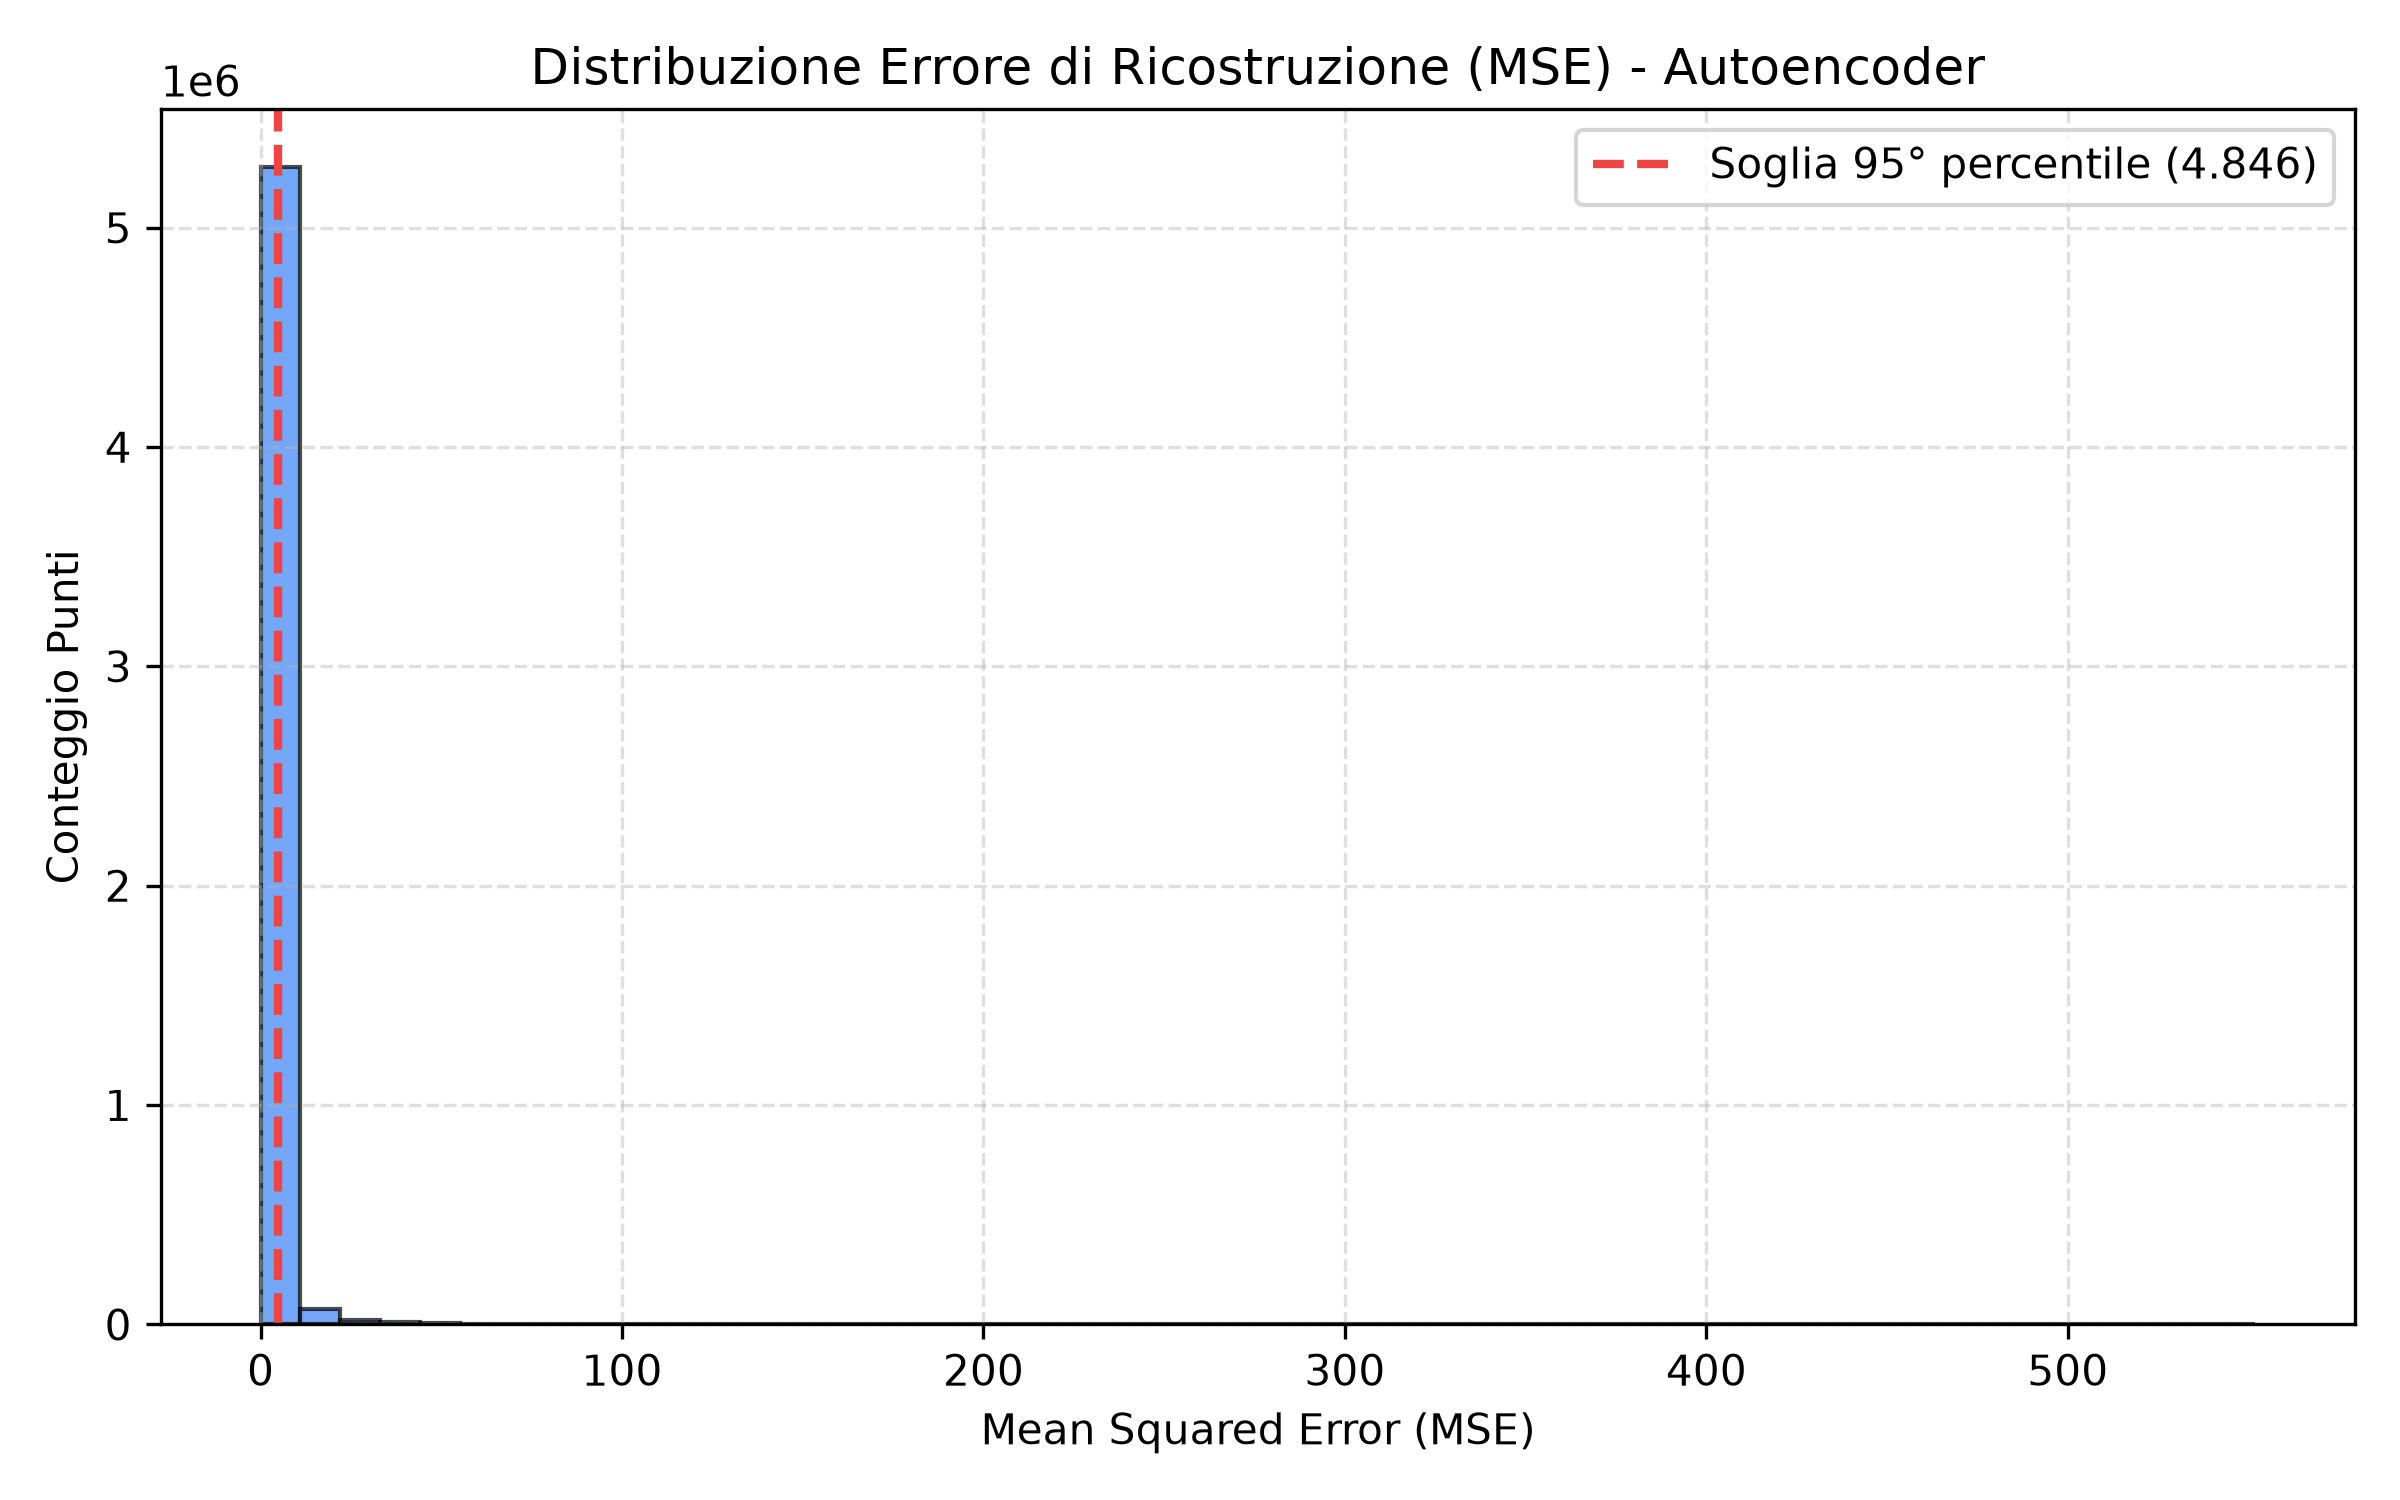
\includegraphics[width=0.82\textwidth]{autoencoder_mse_distribution.png}
    \caption{Distribuzione dell'errore di ricostruzione (MSE) dell'autoencoder con soglia al $95^\circ$ percentile.}
    \label{fig:autoencoder_mse}
\end{figure}

L'efficacia della modellazione neurale trova conferma nell'analisi della distribuzione dell'errore di ricostruzione dell'\textbf{Autoencoder}, illustrata nella Figura~\ref{fig:autoencoder_mse}. La quasi totalità dei punti temporali fisiologicamente stabili si concentra in una campana ristretta con valori di errore quadratico medio prossimi allo zero; al contrario, le configurazioni atipiche generano una marcata coda lunga a destra della distribuzione, superando nettamente la soglia empirica del $95^\circ$ percentile evidenziata dalla linea tratteggiata.

\begin{figure}[ht]
    \centering
    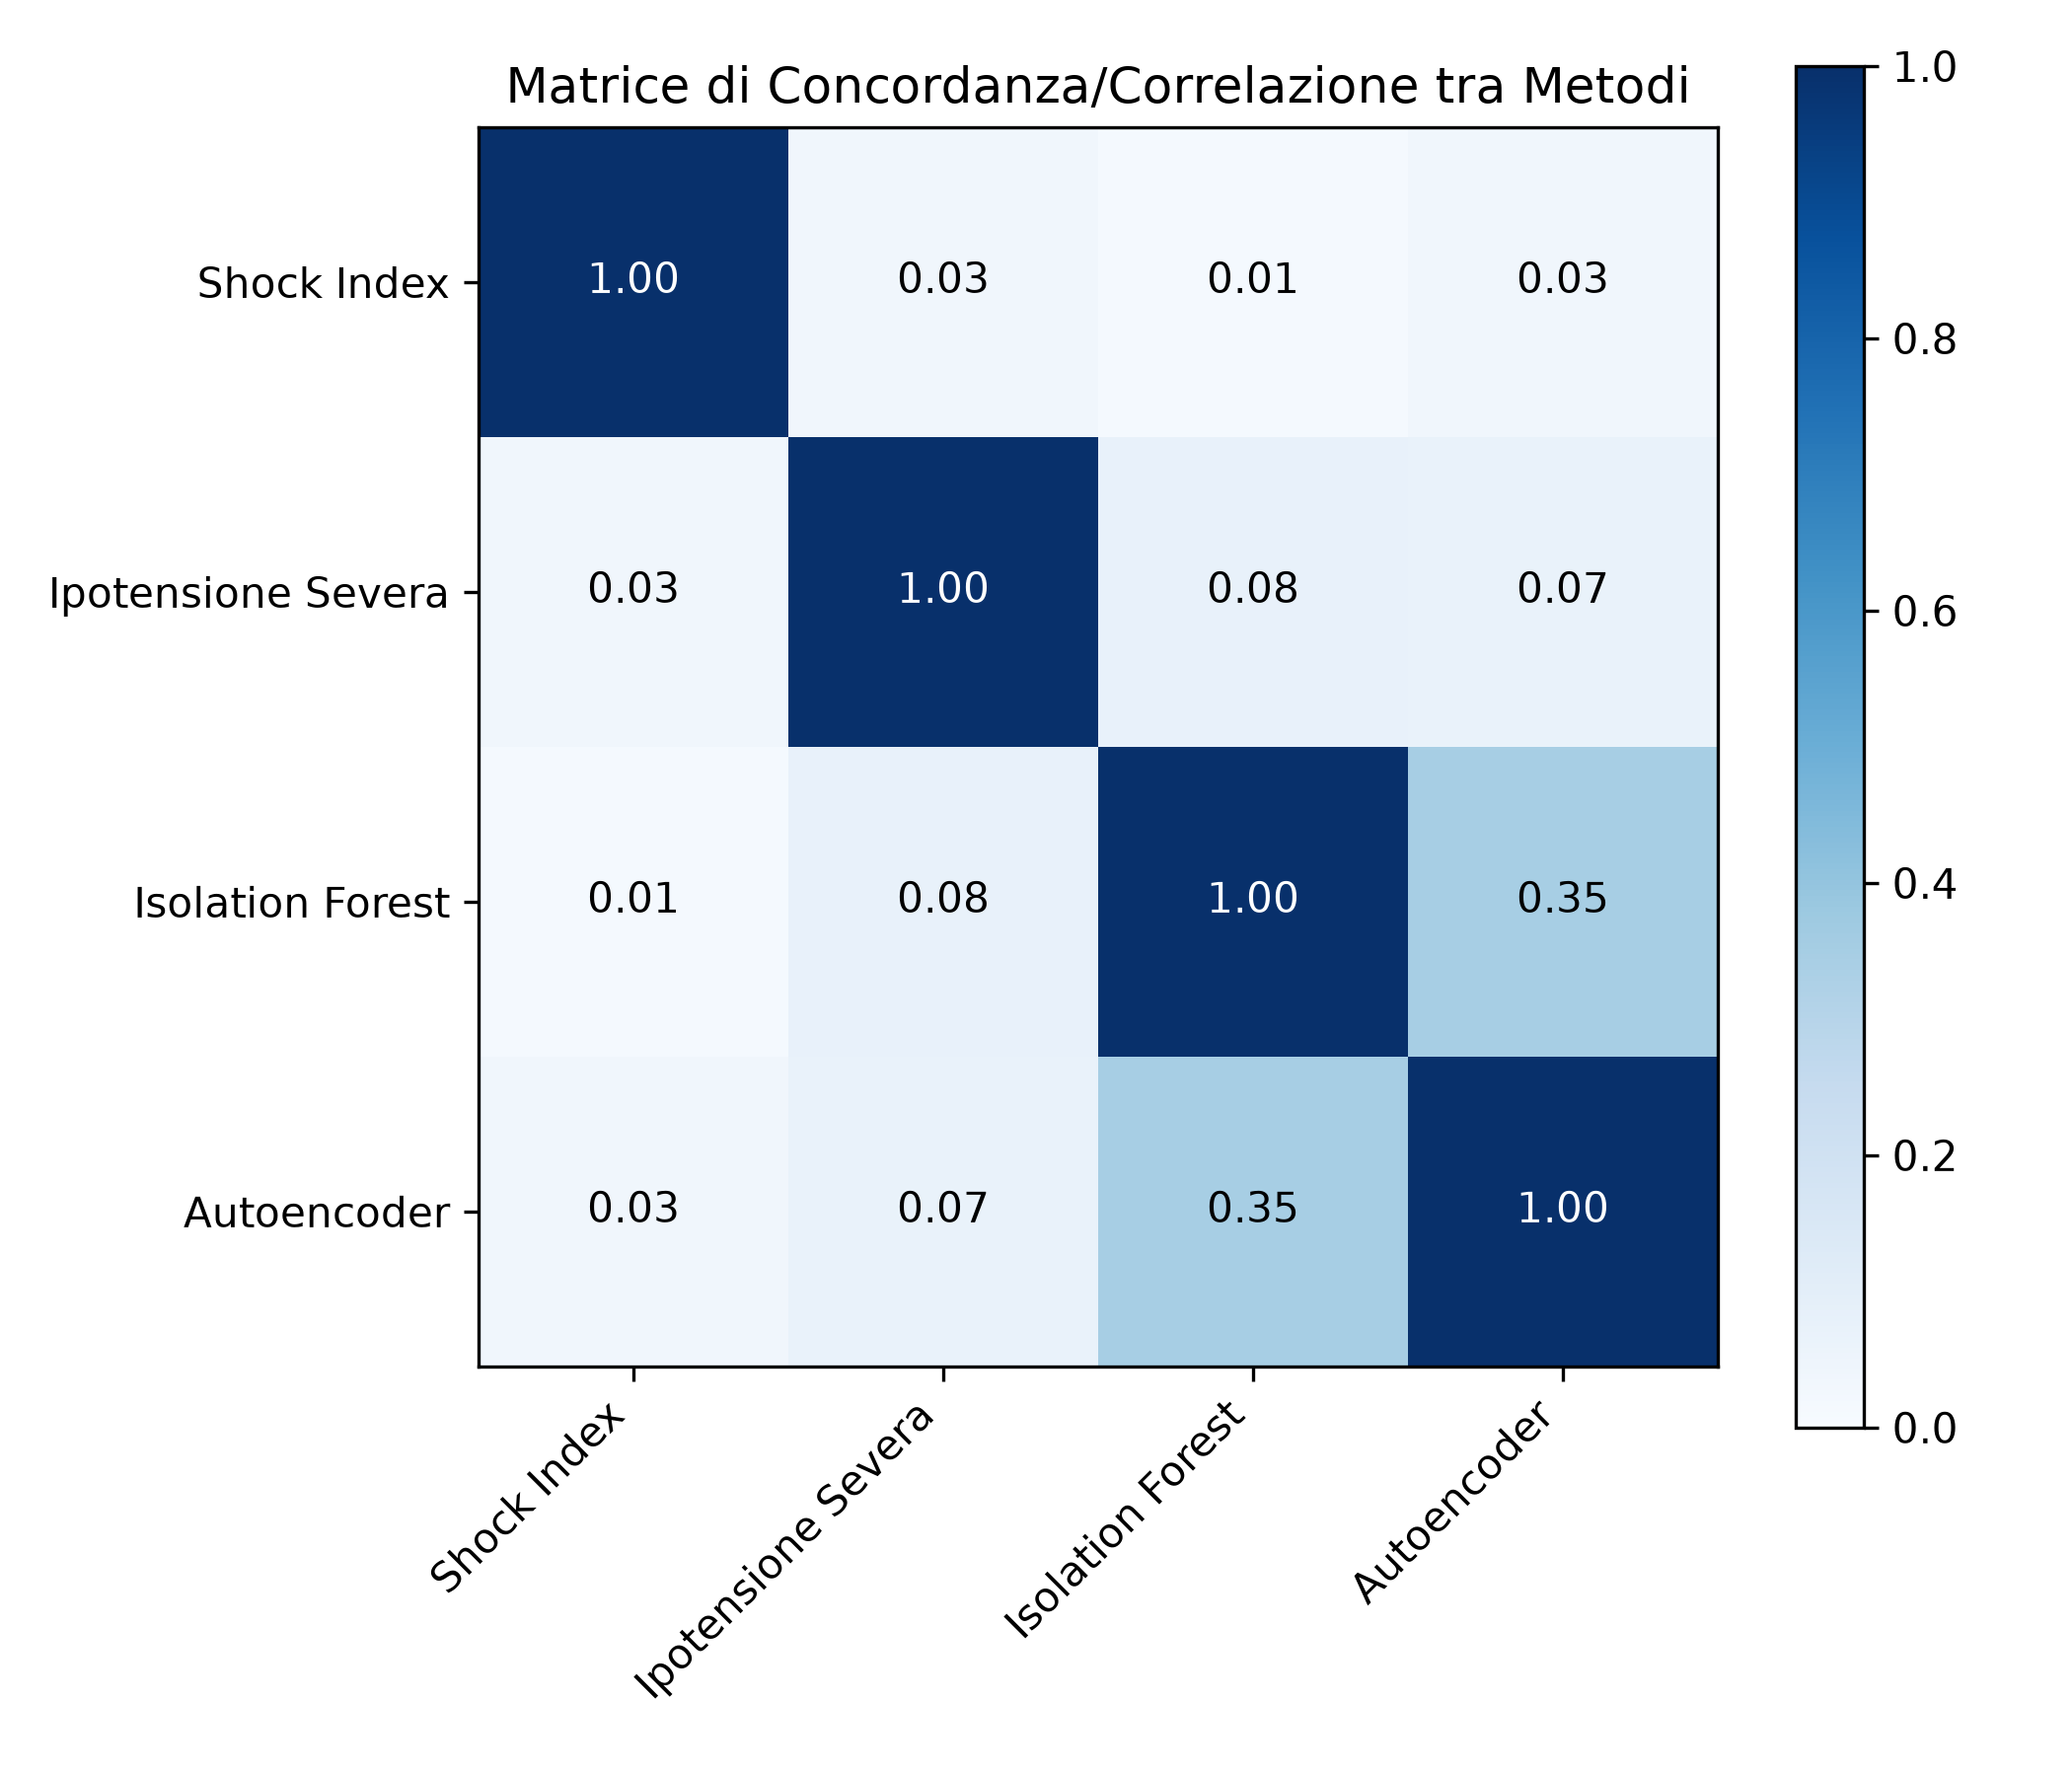
\includegraphics[width=0.76\textwidth]{anomaly_overlap_matrix.png}
    \caption{Matrice di concordanza/correlazione tra le regole cliniche e i modelli ML.}
    \label{fig:overlap_matrix}
\end{figure}

La reciproca interazione tra le quattro metodologie di detection è visualizzata nella matrice di concordanza e correlazione di Figura~\ref{fig:overlap_matrix}. Il grafico evidenzia la concordanza positiva esistente tra le regole emodinamiche e i modelli non supervisionati, confermando come l'approccio ibrido multilivello consenta di intersecare la specificità dell'euristica medica con l'ampiezza di copertura del \textbf{machine learning}.

\section{Persistenza e tracciamento delle anomalie su MongoDB}
A completamento del flusso di rilevamento, gli istanti temporali valutati come anomali da almeno una delle quattro metodologie vengono persistiti all'interno della collezione MongoDB denominata \texttt{anomalies\_detected}.

Ciascun documento memorizzato nella collezione raccoglie le seguenti informazioni:
l'identificativo del caso clinico (\texttt{case\_id});
il timestamp esatto in cui si è verificata l'anomalia;
l'array \texttt{methods}, che elenca i nomi degli algoritmi che hanno segnalato l'istante (ad esempio \texttt{["shock\_index", "isolation\_forest"]});
la marcatura temporale di esecuzione \texttt{detected\_at}, che garantisce la tracciabilità dell'elaborazione analitica.

Al fine di garantire l'idempotenza della pipeline e prevenire la presenza di anomalie obsolete nel database, la procedura nello script \texttt{detector.py} cancella preliminarmente tutti i riscontri pregressi associati al caso clinico esaminato prima di registrare i nuovi risultati. Tale accorgimento assicura che, qualora una successiva esecuzione su un paziente stabilizzato non rilevi alcuna anomalia, le segnalazioni storiche vengano rimosse correttamente senza lasciare falsi allarmi nella base di dati.
